\chapter{Theoretical Framework}

\begin{figure}[h]
    \centering
    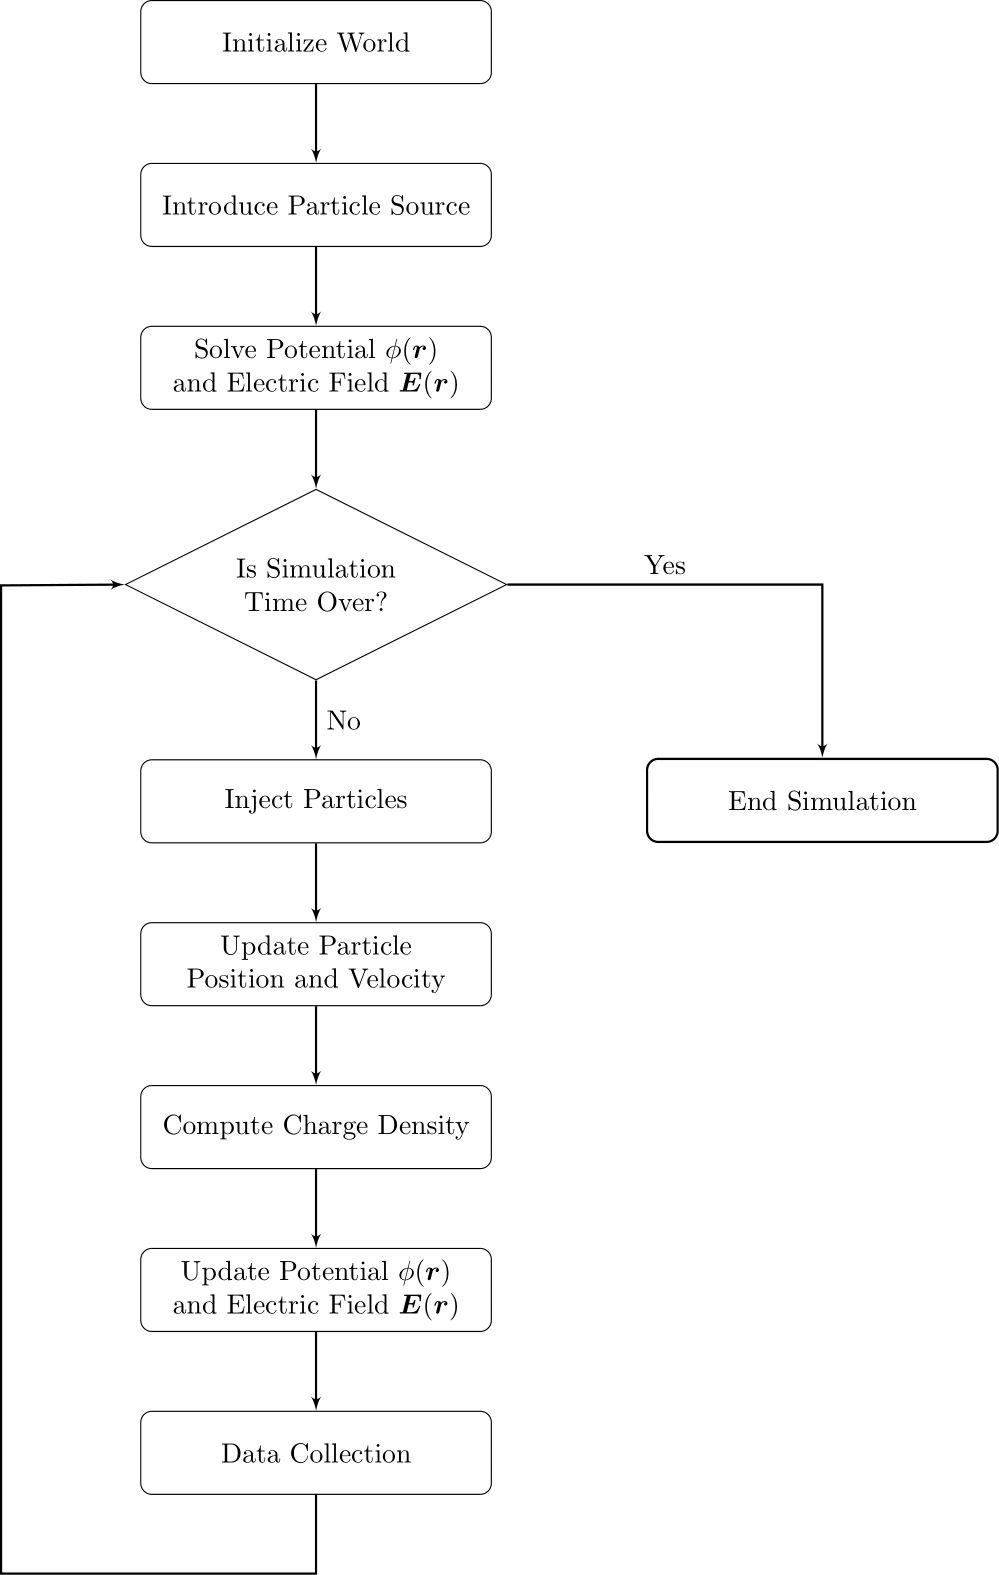
\includegraphics[width=0.7\linewidth]{figures/chapter 2/Flowchart_Studienprojekt-1.png}
    \caption{Caption}
    \label{fig:enter-label}
\end{figure}

\section{Lorentz Force}

\section{Maxwells Equations}

\subsection{Poisson Equation}

\section{Discretize World Domain}

\section{Potential Solver}

\subsection{Gauss Seidel}

\subsection{Seccesive Over Relaxation}

\section{Electric Field Solver}

\section{Particle Motion}

\subsection{Leapfrog Method}

\subsection{Interpolation}

\section{Introduction Particle Sources}

\subsection{Quiet Start method}

